\documentclass{beamer}

\usetheme{Madrid}
\usecolortheme{default}

\usepackage[utf8]{inputenc}
\usepackage[T1]{fontenc}
\usepackage{lmodern}
\usepackage{graphicx}
\graphicspath{{../../assets/}}
\usepackage{tikz}

\title[MidTerm (HO14)]{Sistema Bancario TCP Multithread}
\subtitle{Hands-On 14 - MidTerm}
\author{Massimo Mantineo (541924)}
\institute[Unime]{Università degli Studi di Messina}
\date{A.A. 2024/2025}

\begin{document}

\begin{frame}
  \titlepage
\end{frame}

\begin{frame}{Indice}
  \tableofcontents
\end{frame}

\section{Introduzione al problema}
\begin{frame}{Introduzione al problema}
  \textbf{Obiettivo del MidTerm}
  \vspace{0.5cm}
  
  Sviluppare un sistema client-server bancario per un singolo correntista.
  \begin{itemize}
      \item \textbf{Protocollo}: TCP (garanzia di consegna e ordine).
      \item \textbf{Accessi Concorrenti}: E-banking, App, Terminale, ecc.
      \item \textbf{Limiti Strutturali}: Massimo 10 connessioni threads globali simultanee elaborabili per volta per non sovraccaricare il server.
      \item \textbf{Operazioni Supportate}: CRUD su memoria volatile (ADD, DELETE, UPDATE, LIST).
  \end{itemize}
\end{frame}

\section{Stato dell'arte}
\begin{frame}{Stato dell'arte}
  \textbf{Le Componenti del Networking}
  \vspace{0.3cm}
  
  \begin{itemize}
      \item \textbf{TCP Sockets}: Modello di elaborazione che richiede \texttt{bind}, \texttt{listen} ed \texttt{accept}.
      \item \textbf{Paradigma Demultiplexer}: Il socket server master ha il solo scopo di instradare. Rilascia per ogni richiesta un nuovo file descriptor virtuale allocato specificatamente per il worker.
      \item \textbf{Race Conditions e Thread Safety}: I threads condividono il medesimo spazio di memoria dell'eseguibile master. Leggere e modificare simultaneamente la base di dati genererà inevitabilmente corruzioni in memoria. 
  \end{itemize}
\end{frame}

\section{Metodologia usata}
\begin{frame}{Metodologia e Implementazione - 1}
  \textbf{Strutturazione Backend C}
  
  \vspace{0.3cm}
  \begin{itemize}
      \item Un array esteso \texttt{Transaction db[MAX\_RECORDS]} opera da surrogato al database relazionale.
      \item Si utilizza un semaforo contatore (\texttt{sem\_t limiter}) posizionato a limite 10. Viene chiamata la \texttt{wait()} prima della \texttt{accept()} per interdire nuovi allocamenti ad array già pieno.
      \item In fase di chiusura socket del client nel demone (\texttt{QUIT}), la chiamata a \texttt{post()} ripulisce il posto.
  \end{itemize}
\end{frame}

\begin{frame}{Metodologia e Implementazione - 2}
  \textbf{L'imperativo della Mutua Esclusione}
  
  \vspace{0.3cm}
  L'assoluta stabilità dei dati è garantita dal \textit{Mutex}:
  \begin{itemize}
      \item Quando stringiamo i comandi testuali tramite \texttt{sscanf}, filtriamo l'input.
      \item Prima di scorrere il database (\texttt{for loop}), \textbf{acquisiamo il lock}.
      \item In base al target (\textit{Aggiunta, Rimozione o Modifica per ID}), salviamo il match, verifichiamo la clausola \textit{Active = 1 o 0} della struct.
      \item \textbf{Rilasciamo il lock} solo a manipolazione della memoria conclusa, o durante un ritorno di Errore.
  \end{itemize}
\end{frame}

\section{Risultati sperimentali}
\begin{frame}[fragile]{Risultati sperimentali}
  Testato con successo su terminale locale \texttt{127.0.0.1}.
  \vspace{0.3cm}
  
\begin{verbatim}
--- Connected to Bank Server ---
BANK> ADD 101 25.50 Ricarica Prepagata
OK: ADDED 101
BANK> LIST
--- TRANSACTION LIST ---
[101] 25.50 - Ricarica Prepagata
------------------------
\end{verbatim}

  Dimostrata anche la stabilità su accessi paralleli inviando in stallo il lock per emulazione. Nessun crash verificato.
\end{frame}

\begin{frame}{Analisi del Traffico (Wireshark)}
  \textbf{3-Way Handshake TCP}
  \vspace{0.2cm}

  \begin{figure}[H]
      \centering
      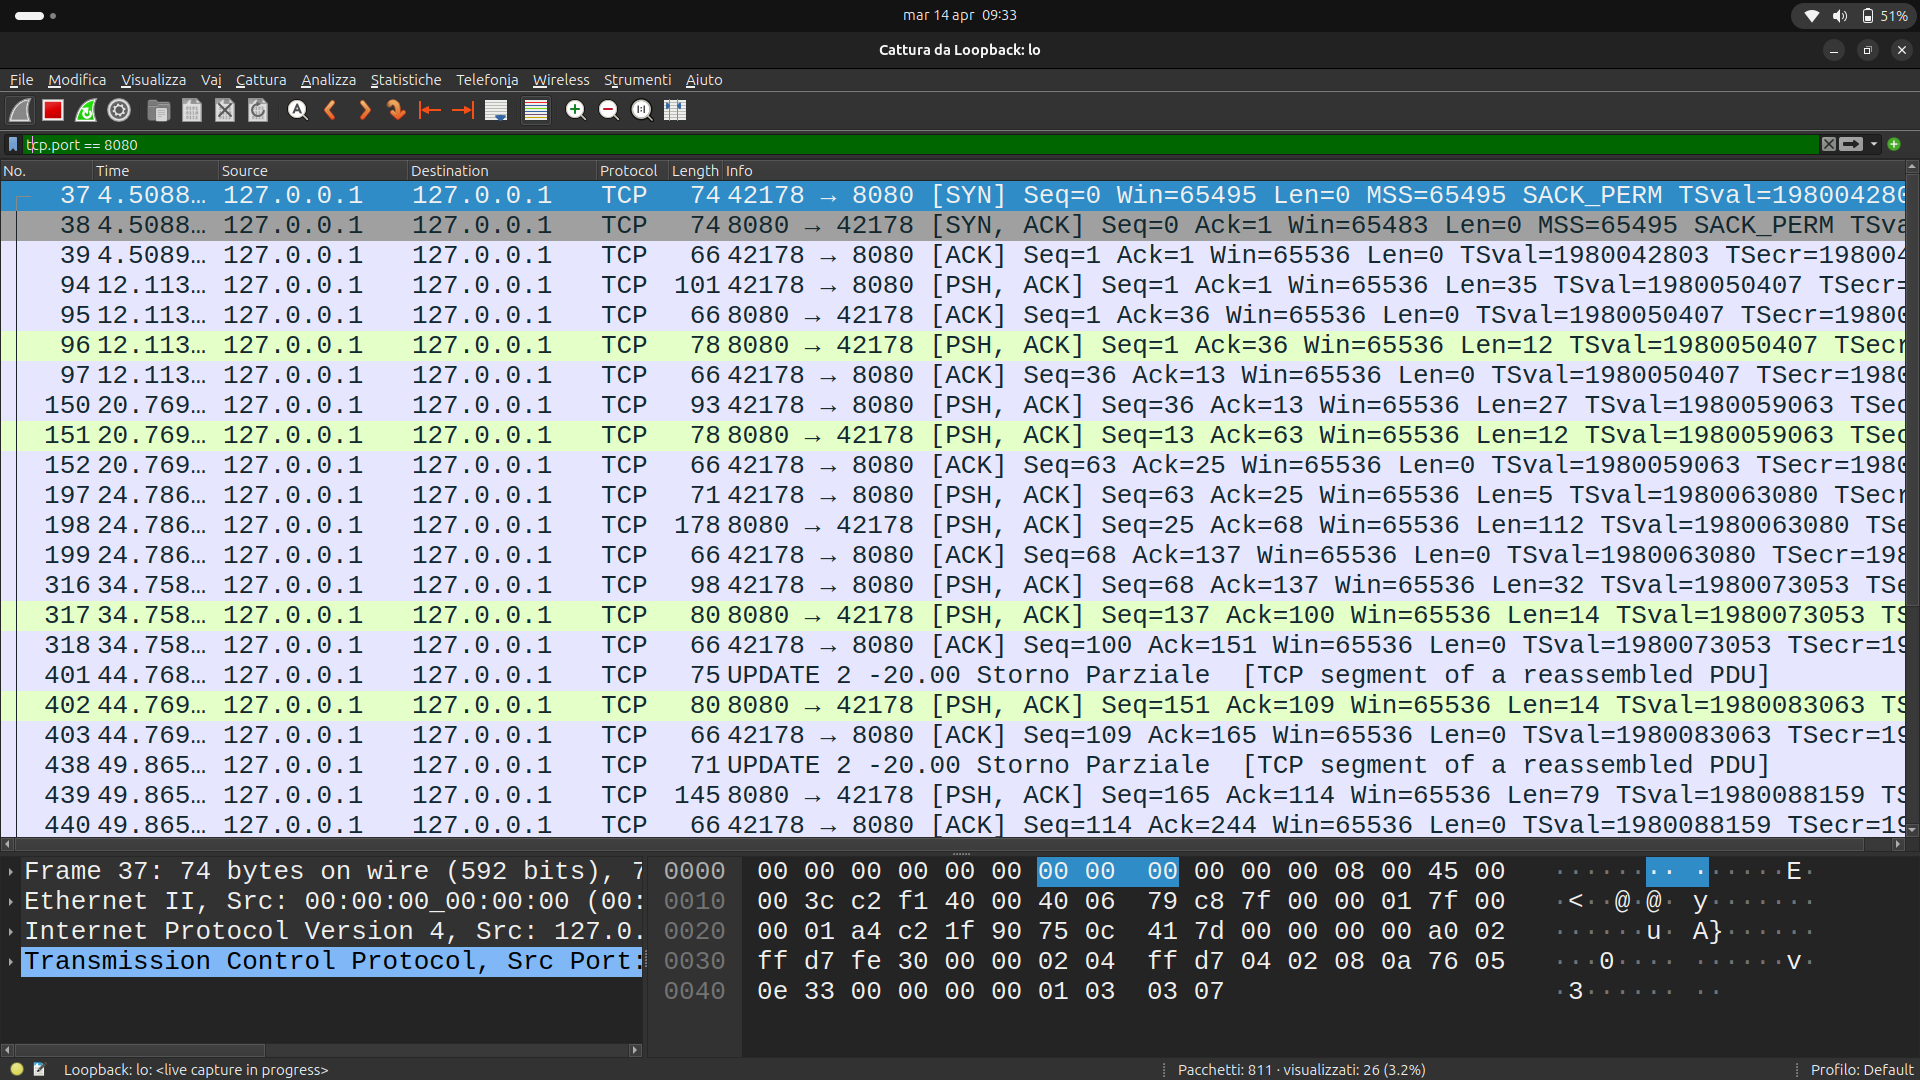
\includegraphics[width=0.9\textwidth]{ho14/image.png}
  \end{figure}

  \begin{itemize}
      \item Instaurazione canale tramite \texttt{[SYN]}, \texttt{[SYN, ACK]}, \texttt{[ACK]}.
      \item Trasferimento payload operativo segnalato via \texttt{[PSH, ACK]}.
      \item Teardown elegante a fine lavoro tramite flag \texttt{[FIN, ACK]}.
  \end{itemize}
\end{frame}

\section{Conclusione e sviluppi futuri}
\begin{frame}{Conclusione e sviluppi futuri}
  \textbf{Conclusioni:}
  Il codice sviluppato implementa un \textit{Proof of Concept} robusto ed espandibile senza l'overhead di strutture applicative gravose.

  \vspace{0.5cm}
  \textbf{Prospettive di Sviluppo Futuro:}
  \begin{itemize}
      \item \textbf{Database Reale}: Sostituzione dell'array RAM con \texttt{SQLite/MariaDB} richiamati via Drivers C SQL per garantire persistenza (\textit{Durability}).
      \item \textbf{Thread Pool}: Abbandono dei \textit{Detached Threads} grezzi a favore di un pool pre-allocato di 10 worker, che estraggono i file-descriptor tramite coda (pattern Produttore-Consumatore appreso in HO12).
  \end{itemize}
\end{frame}

\begin{frame}
  \centering
  \Huge \textbf{Grazie per l'attenzione!}
\end{frame}

\end{document}
